% Template PNSAC newsletter - Article
% Language: Latex
%

% Head

\title{70th Anniversary of first Canadian Non-stop Transcontinental Flight
}
\author{Roger Button}

\maketitle

%\end{multicols}

"If some countries have too much history, we have too much geography" said
former Prime Minister William Lyon Mackenzie King, to the House of Commons in
1936. He would not have known at the time that some thirteen years later an
aviation event would take place that would help to shrink this geography.

January 15, 1949 was a noticeable day in the history of Canadian aviation. On
that day the first non-stop transcontinental flight was made. The aircraft was
Royal Canadian Air Force North Star, registration number 17512. It was operated
by 426 Thunderbird Squadron which was stationed at Dorval, QC. The aircraft was
captained by F/O J.A.F. Jolicoeur and crewed by 14 members of the Experimental
and Proving Establishment from RCAF Rockcliffe.

\begin{figure}[ht!]
   \vspace{2em}
   \centering
   %name of the graphic, without the path AND in EPS format:
   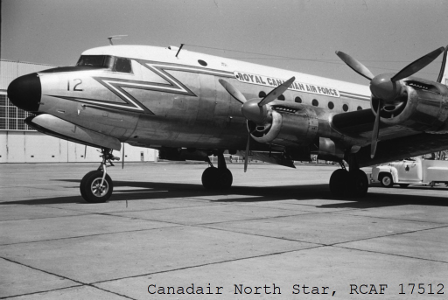
\includegraphics[scale=0.5]{nstar-212-scaled.png}
   %caption of the figure 
   \caption*{\small \em North Star 17512}
   %label of the figure, which has to correspond to \ref{}:
   \label{fig:nstar-17515}
\end{figure}

While 17512 was relatively new to the RCAF it had been one of the earliest
aircraft to roll off the Canadair Assembly line at Cartierville, QC in 1946.
However, instead of going directly into service with the RCAF it, along with
six other aircraft were loaned to Trans Canada Airlines (later to become Air
Canada). It was was not until 1948 that the aircraft was taken on strength by
426 Squadron.

The aircraft had a maximum range of 3,060 miles. This allowed 17512 to make the
non-stop flight from Vancouver to Halifax a distance of 2,785 miles. The flight
took eight hours and thirty two minutes. A year later the aircraft bested its
time by making the same journey in eight hours and twenty five minutes.

While the flight was an aviation first, it was also another step in the history
of transcontinental travel in Canada. This started with arrival of the famous
Scottish explorer Sir Alexander Mckenzie at the Pacific Ocean on July 22, 1793.
He became the first European to cross North America north of Mexico. It was
nearly one hundred years later that the next major leap in transcontinental
travel took place with the completion of the Canadian Pacific Railway when the
last spike was driven on November 7, 1885 at Eagle Pass, BC. In October 1920
the Canadian Air Board staged a cross country mail demonstration but this
involved a relay of five aircraft and a total flying time of 49 hours from
Halifax to Vancouver. In 1939 Trans Canada Airlines flew the first commercial
transcontinental flight from Toronto to Vancouver in 16 hours with four stops.
The airline, however, didn't launch a non-stop transcontinental flight between
the same airports until June 1, 1957. The flight also took eight hours and
thirty two minutes using a Super Constellation. This was same time, to the
minute, that the North Star took eight years earlier and on a longer route.







\begin{footnotesize}
    \raggedleft PNSAC\\
\end{footnotesize}

%\begin{multicols}{2}

% End of text.

%%% Local Variables: 
%%% mode: latex
%%% TeX-master: main_document.tex
%%% End: 

